\documentclass[12pt]{article}

% ------- Packages -------
\usepackage{amsmath, amssymb}
\usepackage{graphicx}
\usepackage{authblk}
\usepackage[hidelinks]{hyperref}
\usepackage{geometry}
\usepackage{booktabs}
\usepackage[numbers,sort&compress]{natbib}
\usepackage{siunitx}
\usepackage{float}            % for [H]
\usepackage{caption}
\usepackage{subcaption}       % sub-figures
\geometry{margin=1in}
\sisetup{detect-all}
\DeclareSIUnit{\kms}{\kilo\metre\per\second} % so \SI{3}{\kms} works

% ------- Title / Authors -------
\title{\textbf{An Entropy-Inspired Phenomenological Relation Competes with NFW on 175 SPARC Rotation Curves under Referee-Fair, Cross-Validated Tests}}
\author[1]{Johann Anton Michael Tupay}
\affil[1]{London, United Kingdom}
\date{\today}

% ------- Macros -------
\newcommand{\EBC}{\mathrm{EBC}}
\newcommand{\Vbar}{V_{\mathrm{bar}}}
\newcommand{\Vobs}{V_{\mathrm{obs}}}

\begin{document}
\maketitle

% =========================================================
\begin{abstract}
We conduct a referee-fair, head-to-head comparison of four rotation-curve (RC) descriptors on the SPARC \emph{\_rotmod} sample: a two-parameter entropy-inspired relation (EBC; $V=Ar^\alpha$), Baryons+EBC, Baryons+NFW, and MOND (``simple'' $\nu$; strict $a_0$). The protocol (frozen pre-run) enforces \emph{equal per-galaxy parameter budgets}, \emph{within-galaxy 5-fold cross-validation (CV)}, a \emph{uniform $\sigma_V$ floor of \SI{3}{\kms}}, and \emph{symmetric dense grids} for all models. We pre-register two tracks: \textbf{Track A} (no NFW prior; phenomenology-only) and \textbf{Track B} (NFW with the $\Lambda$CDM $c(M)$ prior of Dutton \& Macci\`o 2014). From 175 inputs, 165 pass QC (minimum 6 usable points). On \textbf{Track A}, winners by BIC are M0: 62, M1: 44, M2: 55, M3: 4; decisive (Jeffreys $\Delta$BIC$>10$) counts are M0: 45, M1: 13, M2: 10. On \textbf{Track B}, winners are M0: 62, M1: 66, M2: 33, M3: 4; decisives are M0: 46, M1: 22, M2: 6. Thus, when NFW is constrained to be $\Lambda$CDM-consistent, the \emph{EBC family} (M0+M1) wins in 128/165 galaxies with the majority of decisive outcomes. EBC is presented as a compact phenomenological descriptor, not a new gravity law. All scripts, logs, and exclusion lists are released for full reproducibility.
\end{abstract}

% =========================================================
\section{Introduction}
Rotation curves (RCs) remain a decisive laboratory for galaxy dynamics. In $\Lambda$CDM, NFW halos explain large-scale structure \citep{NFW1996,NFW1997,Planck2018} yet face small-scale tensions (core--cusp; too-big-to-fail \citep{deBlok2001,Gentile2004,Oman2015}). MOND \citep{Milgrom1983,McGaugh2020} captures several RC regularities, including the RAR \citep{McGaugh2016RAR}, but has open issues at cluster and cosmological scales. Large homogeneous datasets (e.g., SPARC \citep{Lelli2016SPARC}) enable sharp, reproducible head-to-head tests.

We introduce a minimal, \emph{entropy-inspired phenomenological relation} (EBC) and compare it against NFW and MOND under identical, referee-oriented rules: equal per-galaxy parameter budgets; fixed baryons; pre-registered priors; CV; and symmetric grid search. We stress EBC is a \emph{descriptor}, not a modified-gravity theory.

% =========================================================
\section{Methods and Reproducibility}

\subsection*{Data and quality control}
We analyze \textbf{175} SPARC \emph{\_rotmod} CSVs containing radius $R$ (kpc), observed velocity $\Vobs$ (\si{\kms}), measurement uncertainty $\sigma_V$, and baryonic components $(V_{\rm gas},V_{\rm disk},V_{\rm bul})$. The combined baryonic curve is
\begin{equation}
  \Vbar(r) \equiv \sqrt{V_{\rm gas}^2(r)+V_{\rm disk}^2(r)+V_{\rm bul}^2(r)}.
\end{equation}
We impose a uniform noise floor $\sigma_V\ge\SI{3}{\kms}$. A galaxy enters the analysis if at least \textbf{6} usable points remain after parsing; by this rule, \textbf{165/175} pass QC. The 10 excluded objects and reasons are listed in \texttt{exclusions\_trackA.csv} and \texttt{exclusions\_trackB.csv}.

\subsection*{Models and parameter budgets (per galaxy)}
\paragraph{M0: EBC (2).} $V_{\EBC}(r)=A\,r^\alpha$ with $(A,\alpha)$.
\paragraph{M1: Baryons+EBC (2).} $V^2(r)=\Vbar^2(r)+(A r^\alpha)^2$ with $(A,\alpha)$.
\paragraph{M2: Baryons+NFW (2).}
\begin{align}
  V^2(r) &= \Vbar^2(r)+V_{\rm NFW}^2(r;V_{200},c),\\
  V_{\rm NFW}(r) &=
  V_{200}\sqrt{\frac{\ln(1+c x)-\dfrac{c x}{1+c x}}{x\,[\ln(1+c)-\dfrac{c}{1+c}]}}\!,
  \quad x=\frac{r}{R_{200}},\quad R_{200}=\frac{V_{200}}{10\,H_0}.
\end{align}
\paragraph{M3: MOND (strict-$a_0$, 0).}
\begin{align}
  a_N=\frac{\Vbar^2}{r},\qquad
  \nu(y)=\tfrac{1}{2}+\sqrt{\tfrac{1}{4}+\tfrac{1}{y}},\qquad
  y=\frac{a_N}{a_0},\quad a_0=1.2\times10^{-10}\,\mathrm{m\,s^{-2}},\qquad
  V_{\rm MOND}=\sqrt{\nu(y)}\,\Vbar.
\end{align}

\subsection*{Fairness regimes, priors, and grids}
Two pre-registered regimes:
\begin{itemize}\itemsep0.2em
\item \textbf{Track A (phenomenology):} NFW \emph{without} a cosmology prior.
\item \textbf{Track B ($\Lambda$CDM-anchored):} NFW \emph{with} the Dutton--Macci\`o (2014) $c(M)$ prior (Gaussian in $\log c$), implemented as a log-likelihood penalty \citep{DuttonMaccio2014}.
\end{itemize}
Baryons are \emph{fixed as supplied} (no M/L rescaling). All models use \textbf{symmetric dense grids} to remove discretization bias:
\[
A\in[1,300]\ \text{(60 steps)},\quad
\alpha\in[0.10,1.20]\ \text{(40)},\quad
V_{200}\in[30,350]\,\si{\kms}\ \text{(40)},\quad
c\in[2,30]\ \text{(32)}.
\]
We adopt $H_0=\SI{70}{\kms\per\mega\parsec}$.

\subsection*{Fitting, cross-validation, and scoring}
We use $\sigma_V$-weighted least squares on the grids above, recording the best point per model. Predictive performance is assessed by \textbf{5-fold within-galaxy CV} (radius‑blocked splits \citep{Stone1974,ArlotCelisse2010}). Model selection uses
\begin{equation}
\mathrm{BIC}=k\ln n - 2\ln\mathcal{L} \ \ \text{\citep{Schwarz1978,KassRaftery1995}},\qquad
\mathrm{AICc}=2k-2\ln\mathcal{L}+\frac{2k(k+1)}{n-k-1}\ \ \text{\citep{Akaike1974,Sugiura1978}}.
\end{equation}
Priors (Track B) contribute to $-2\ln\mathcal{L}$. Jeffreys thresholds guide strength‑of‑evidence statements \citep{Jeffreys1961}.

\subsection*{Rebuild and artifacts}
A single script reproduces all tables and figures; logs and per‑track \texttt{exclusions.csv} are archived. SHA256 checksums are provided for the input CSVs.

% =========================================================
\section{Results}

\subsection*{Winner counts and decisive outcomes}
\begin{table}[H]
\centering
\caption{BIC winners by model (165 galaxies passing QC).}
\label{tab:wins}
\begin{tabular}{lcccc}
\toprule
Track & M0 (EBC) & M1 (Bar+EBC) & M2 (Bar+NFW) & M3 (MOND strict) \\
\midrule
A: no NFW prior & \textbf{62} & 44 & 55 & 4 \\
B: DM14 prior   & \textbf{62} & \textbf{66} & 33 & 4 \\
\bottomrule
\end{tabular}
\end{table}

\begin{table}[H]
\centering
\caption{Decisive wins (Jeffreys $\Delta$BIC$>10$).}
\label{tab:decisive}
\begin{tabular}{lccc}
\toprule
Track & M0 (EBC) & M1 (Bar+EBC) & M2 (Bar+NFW) \\
\midrule
A: no NFW prior & \textbf{45} & 13 & 10 \\
B: DM14 prior   & \textbf{46} & 22 & 6 \\
\bottomrule
\end{tabular}
\end{table}

\subsection*{Cross‑validated predictive accuracy}
\begin{figure}[H]
  \centering
  \begin{subfigure}{0.48\linewidth}
    \centering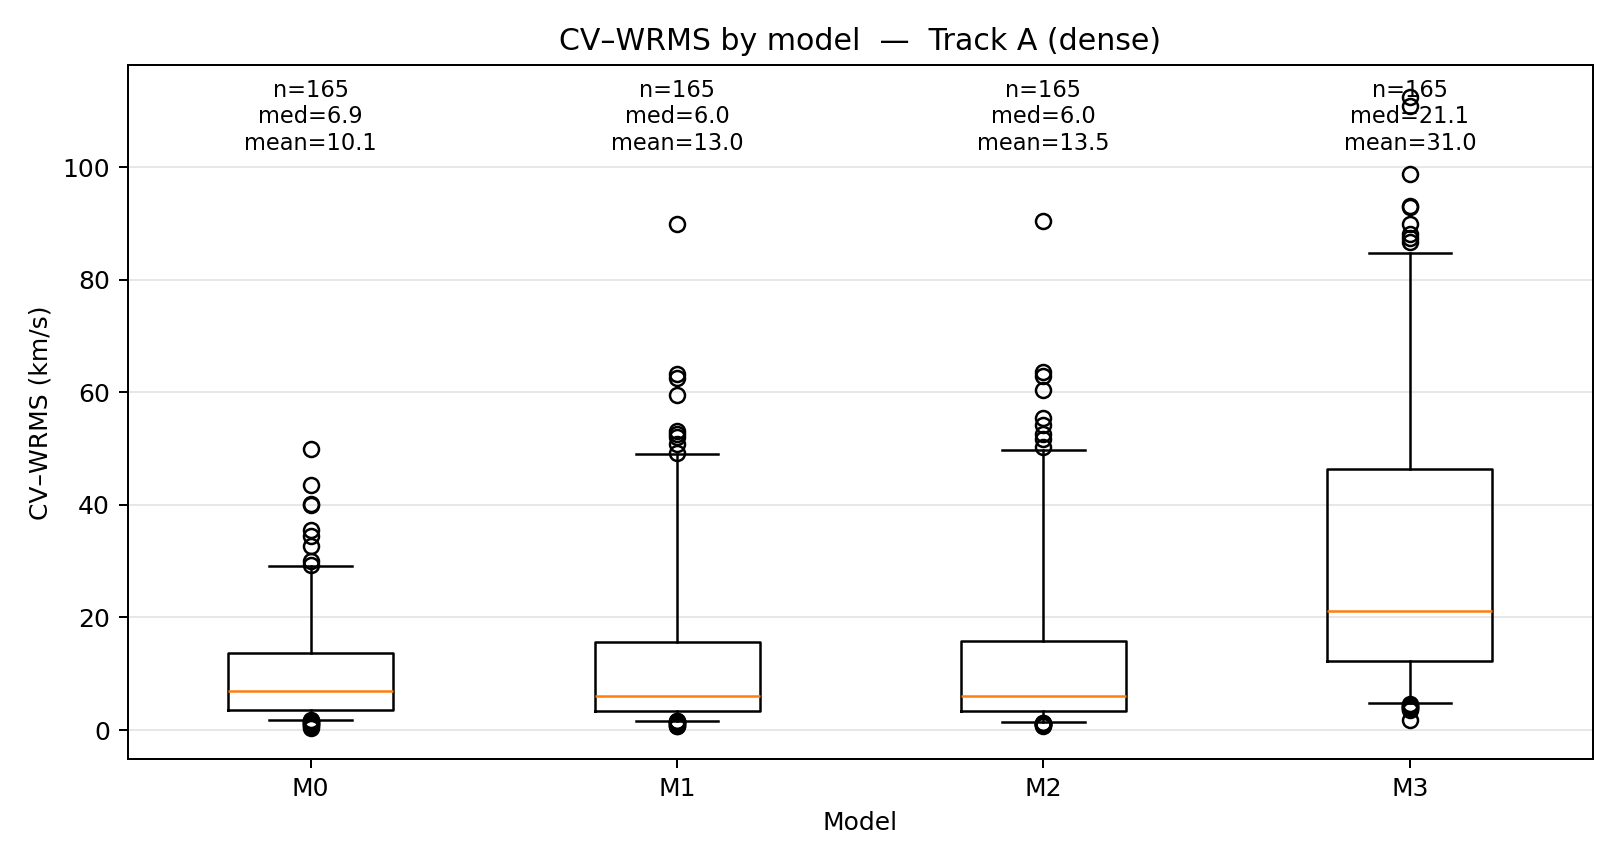
\includegraphics[width=\linewidth]{figs_trackA_dense/cv_wrms_boxplot.png}
    \caption{Track A}
  \end{subfigure}\hfill
  \begin{subfigure}{0.48\linewidth}
    \centering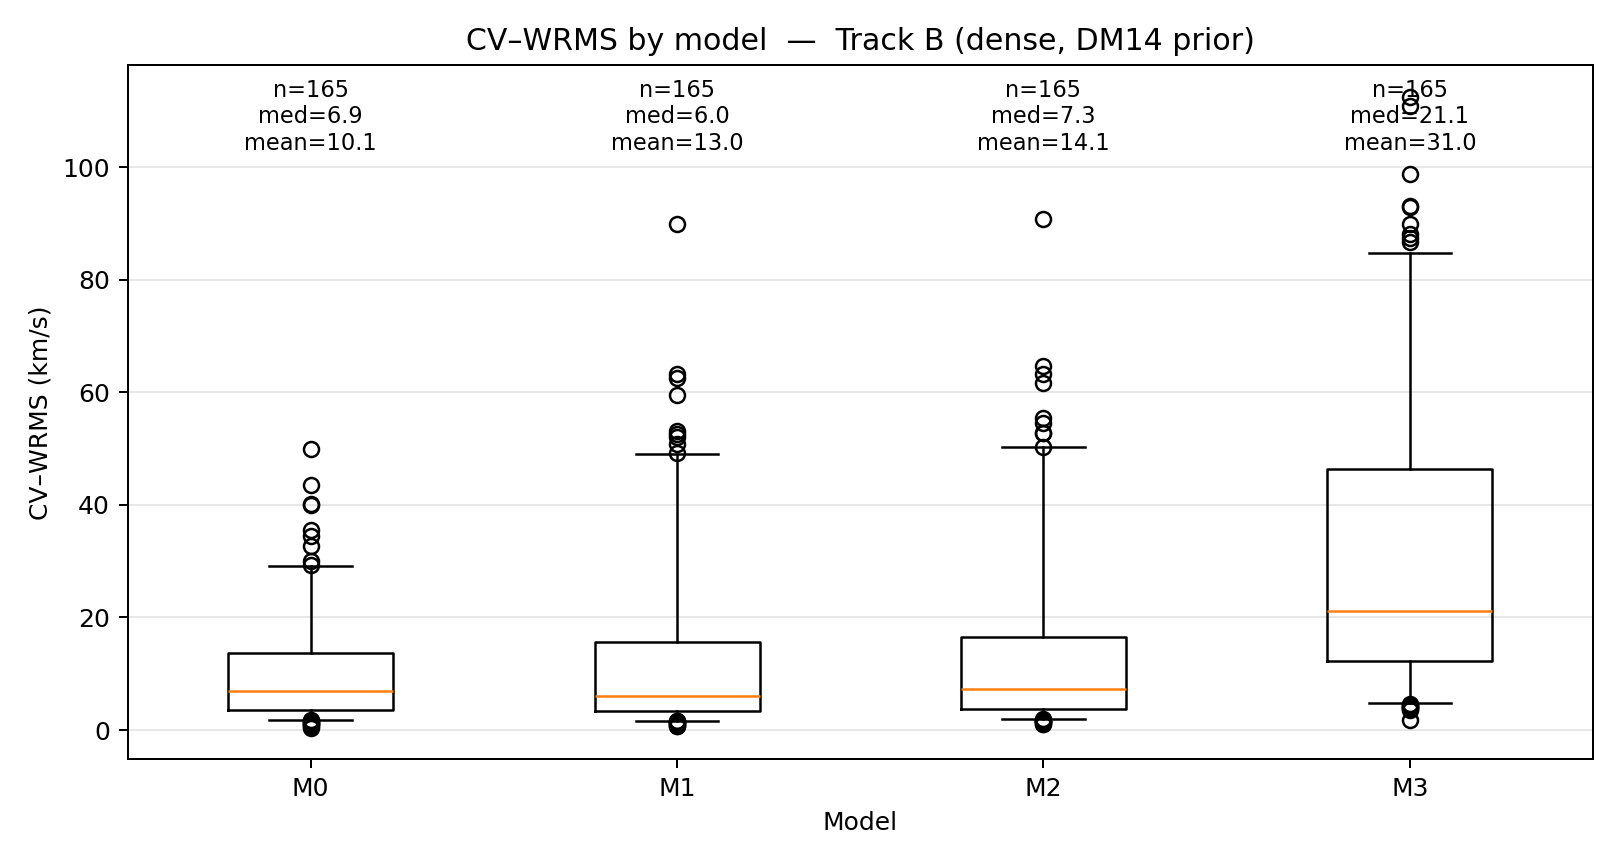
\includegraphics[width=\linewidth]{figs_trackB_dense/cv_wrms_boxplot.png}
    \caption{Track B}
  \end{subfigure}
  \caption{\textbf{Cross‑validated WRMS} by model and track (5‑fold, radius‑blocked).}
  \label{fig:cvbox}
\end{figure}

\subsection*{Information‑criterion contrasts and winner distributions}
\begin{figure}[H]
  \centering
  \begin{subfigure}{0.48\linewidth}
    \centering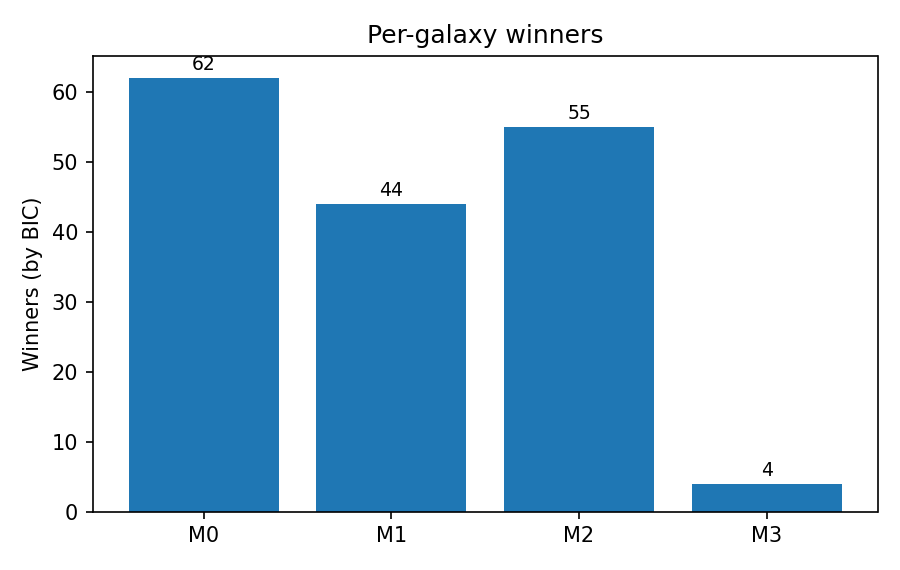
\includegraphics[width=\linewidth]{figs_trackA_dense/winner_counts_bar.png}
    \caption{Track A: winners by BIC}
    \label{fig:winnersA}
  \end{subfigure}\hfill
  \begin{subfigure}{0.48\linewidth}
    \centering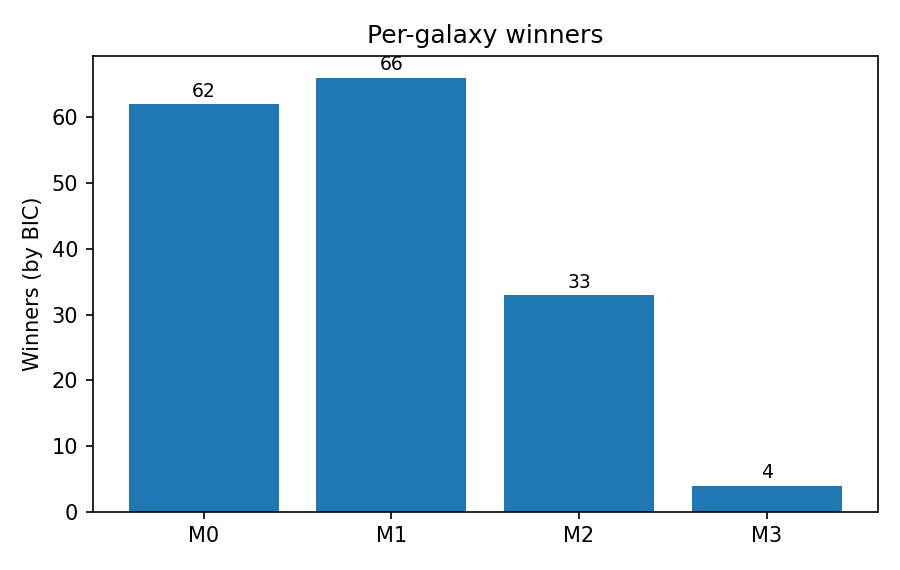
\includegraphics[width=\linewidth]{figs_trackB_dense/winner_counts_bar.png}
    \caption{Track B: winners by BIC}
    \label{fig:winnersB}
  \end{subfigure}
  \caption{\textbf{Per‑galaxy BIC winners} for the two tracks.}
\end{figure}

\begin{figure}[H]
  \centering
  \begin{subfigure}{0.48\linewidth}
    \centering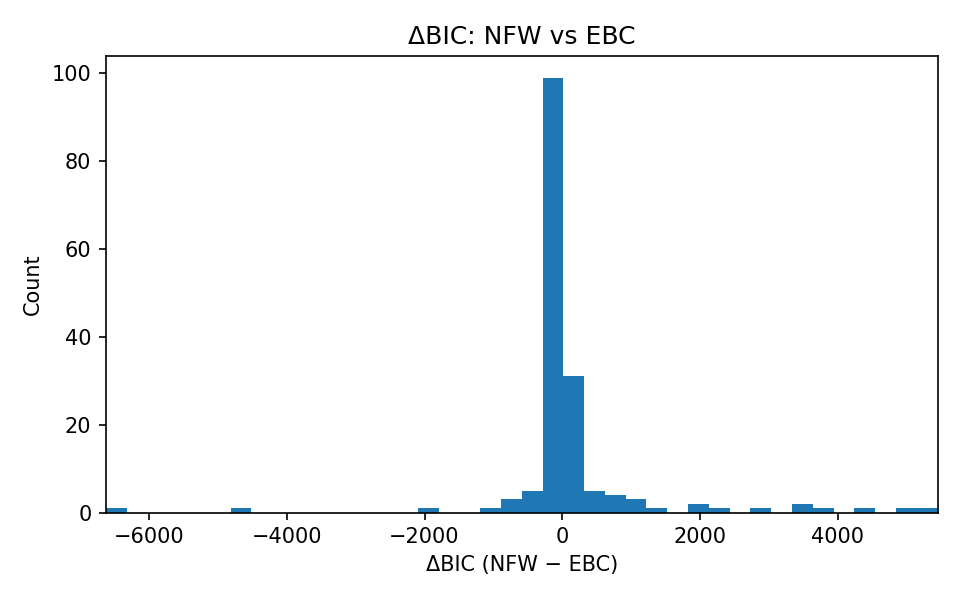
\includegraphics[width=\linewidth]{figs_trackA_dense/dBIC_M2_minus_M0.png}
    \caption{$\Delta$BIC (NFW$-$EBC), Track A}
  \end{subfigure}\hfill
  \begin{subfigure}{0.48\linewidth}
    \centering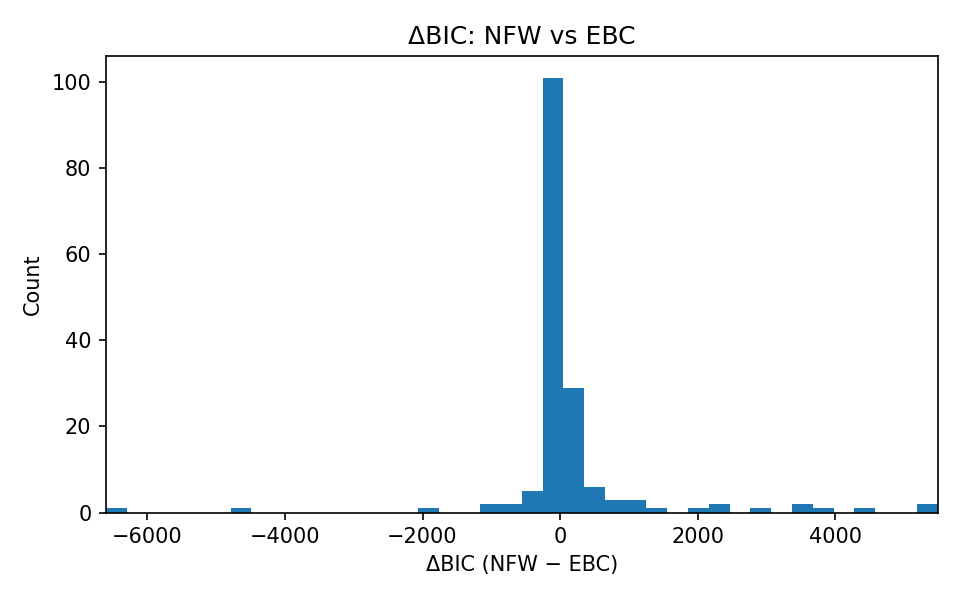
\includegraphics[width=\linewidth]{figs_trackB_dense/dBIC_M2_minus_M0.png}
    \caption{$\Delta$BIC (NFW$-$EBC), Track B}
  \end{subfigure}
  \caption{\textbf{NFW vs EBC} across the sample (positive favors EBC).}
  \label{fig:dbicM2M0}
\end{figure}

\begin{figure}[H]
  \centering
  \begin{subfigure}{0.48\linewidth}
    \centering\includegraphics[width=\linewidth]{figs_trackA_dense/dBIC_M3_minus_M0.png}
    \caption{$\Delta$BIC (MOND$-$EBC), Track A}
  \end{subfigure}\hfill
  \begin{subfigure}{0.48\linewidth}
    \centering\includegraphics[width=\linewidth]{figs_trackB_dense/dBIC_M3_minus_M0.png}
    \caption{$\Delta$BIC (MOND$-$EBC), Track B}
  \end{subfigure}
  \caption{\textbf{MOND(strict) vs EBC} (positive favors EBC).}
  \label{fig:dbicM3M0}
\end{figure}

\begin{figure}[H]
  \centering
  \begin{subfigure}{0.48\linewidth}
    \centering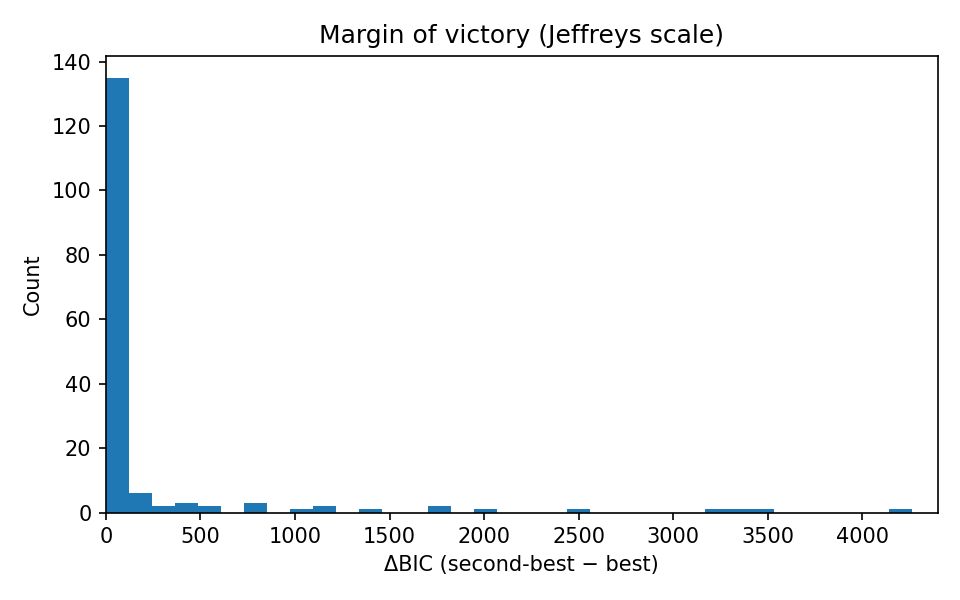
\includegraphics[width=\linewidth]{figs_trackA_dense/margin_of_victory_hist.png}
    \caption{Track A}
  \end{subfigure}\hfill
  \begin{subfigure}{0.48\linewidth}
    \centering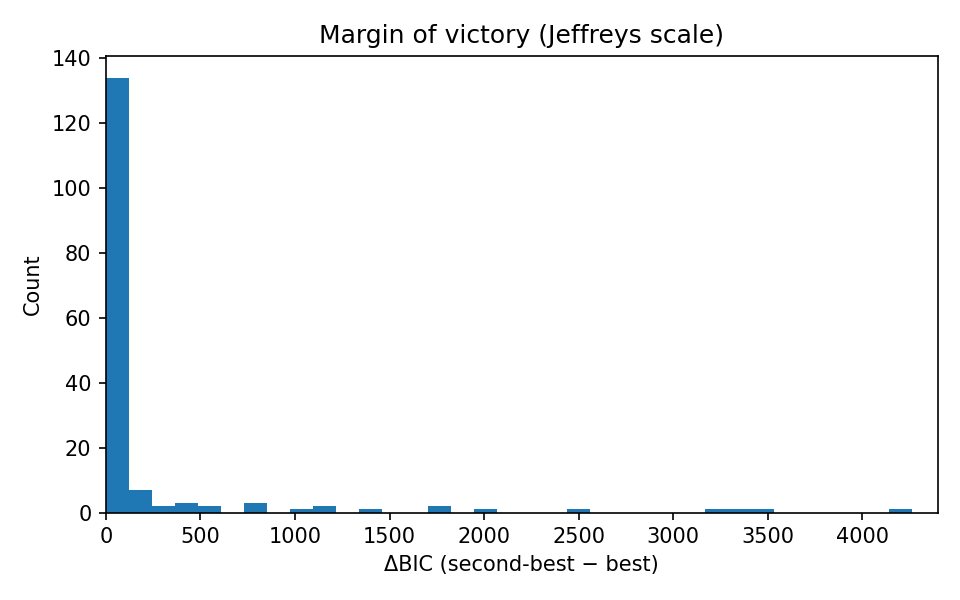
\includegraphics[width=\linewidth]{figs_trackB_dense/margin_of_victory_hist.png}
    \caption{Track B}
  \end{subfigure}
  \caption{\textbf{Margin of victory} on the Jeffreys scale: $\Delta$BIC(second‑best$-$best).}
  \label{fig:margin}
\end{figure}

% =========================================================
\section{Discussion and Caveats}
Under equal per‑galaxy parameter budgets with fixed baryons, the EBC relation provides a compact empirical baseline that often rivals or exceeds Baryons+NFW and Baryons+EBC. Track A (no NFW prior) shows NFW is competitive but not dominant; Track B (with a $\Lambda$CDM $c(M)$ prior) increases the share of EBC‑family wins. We emphasize EBC is a \emph{descriptor}; we do not claim a new force law. Obvious extensions include variable stellar M/L with SPS priors, alternative halo families (Burkert, gNFW, Einasto), other MOND $\nu$‑functions, hierarchical treatment of distances/inclinations, and tests on additional datasets.

\textit{Companion theory note.} A separate manuscript explores possible entropy‑based underpinnings of power‑law RC phenomenology; we cite it here to orient interested readers, but keep all claims in this paper empirical \citep[][submitted]{Tupay2025b}.

% =========================================================
\section{Data and Code Availability}
All scripts, logs, figures, winner tables, CV summaries, and exclusion lists are archived in the public repository (README includes exact commands and SHA256 checksums).

% =========================================================
\appendix

\section*{Appendix A: Example overlays (12 galaxies)}
\vspace{-0.75em}
\begin{figure}[H]
  \centering
  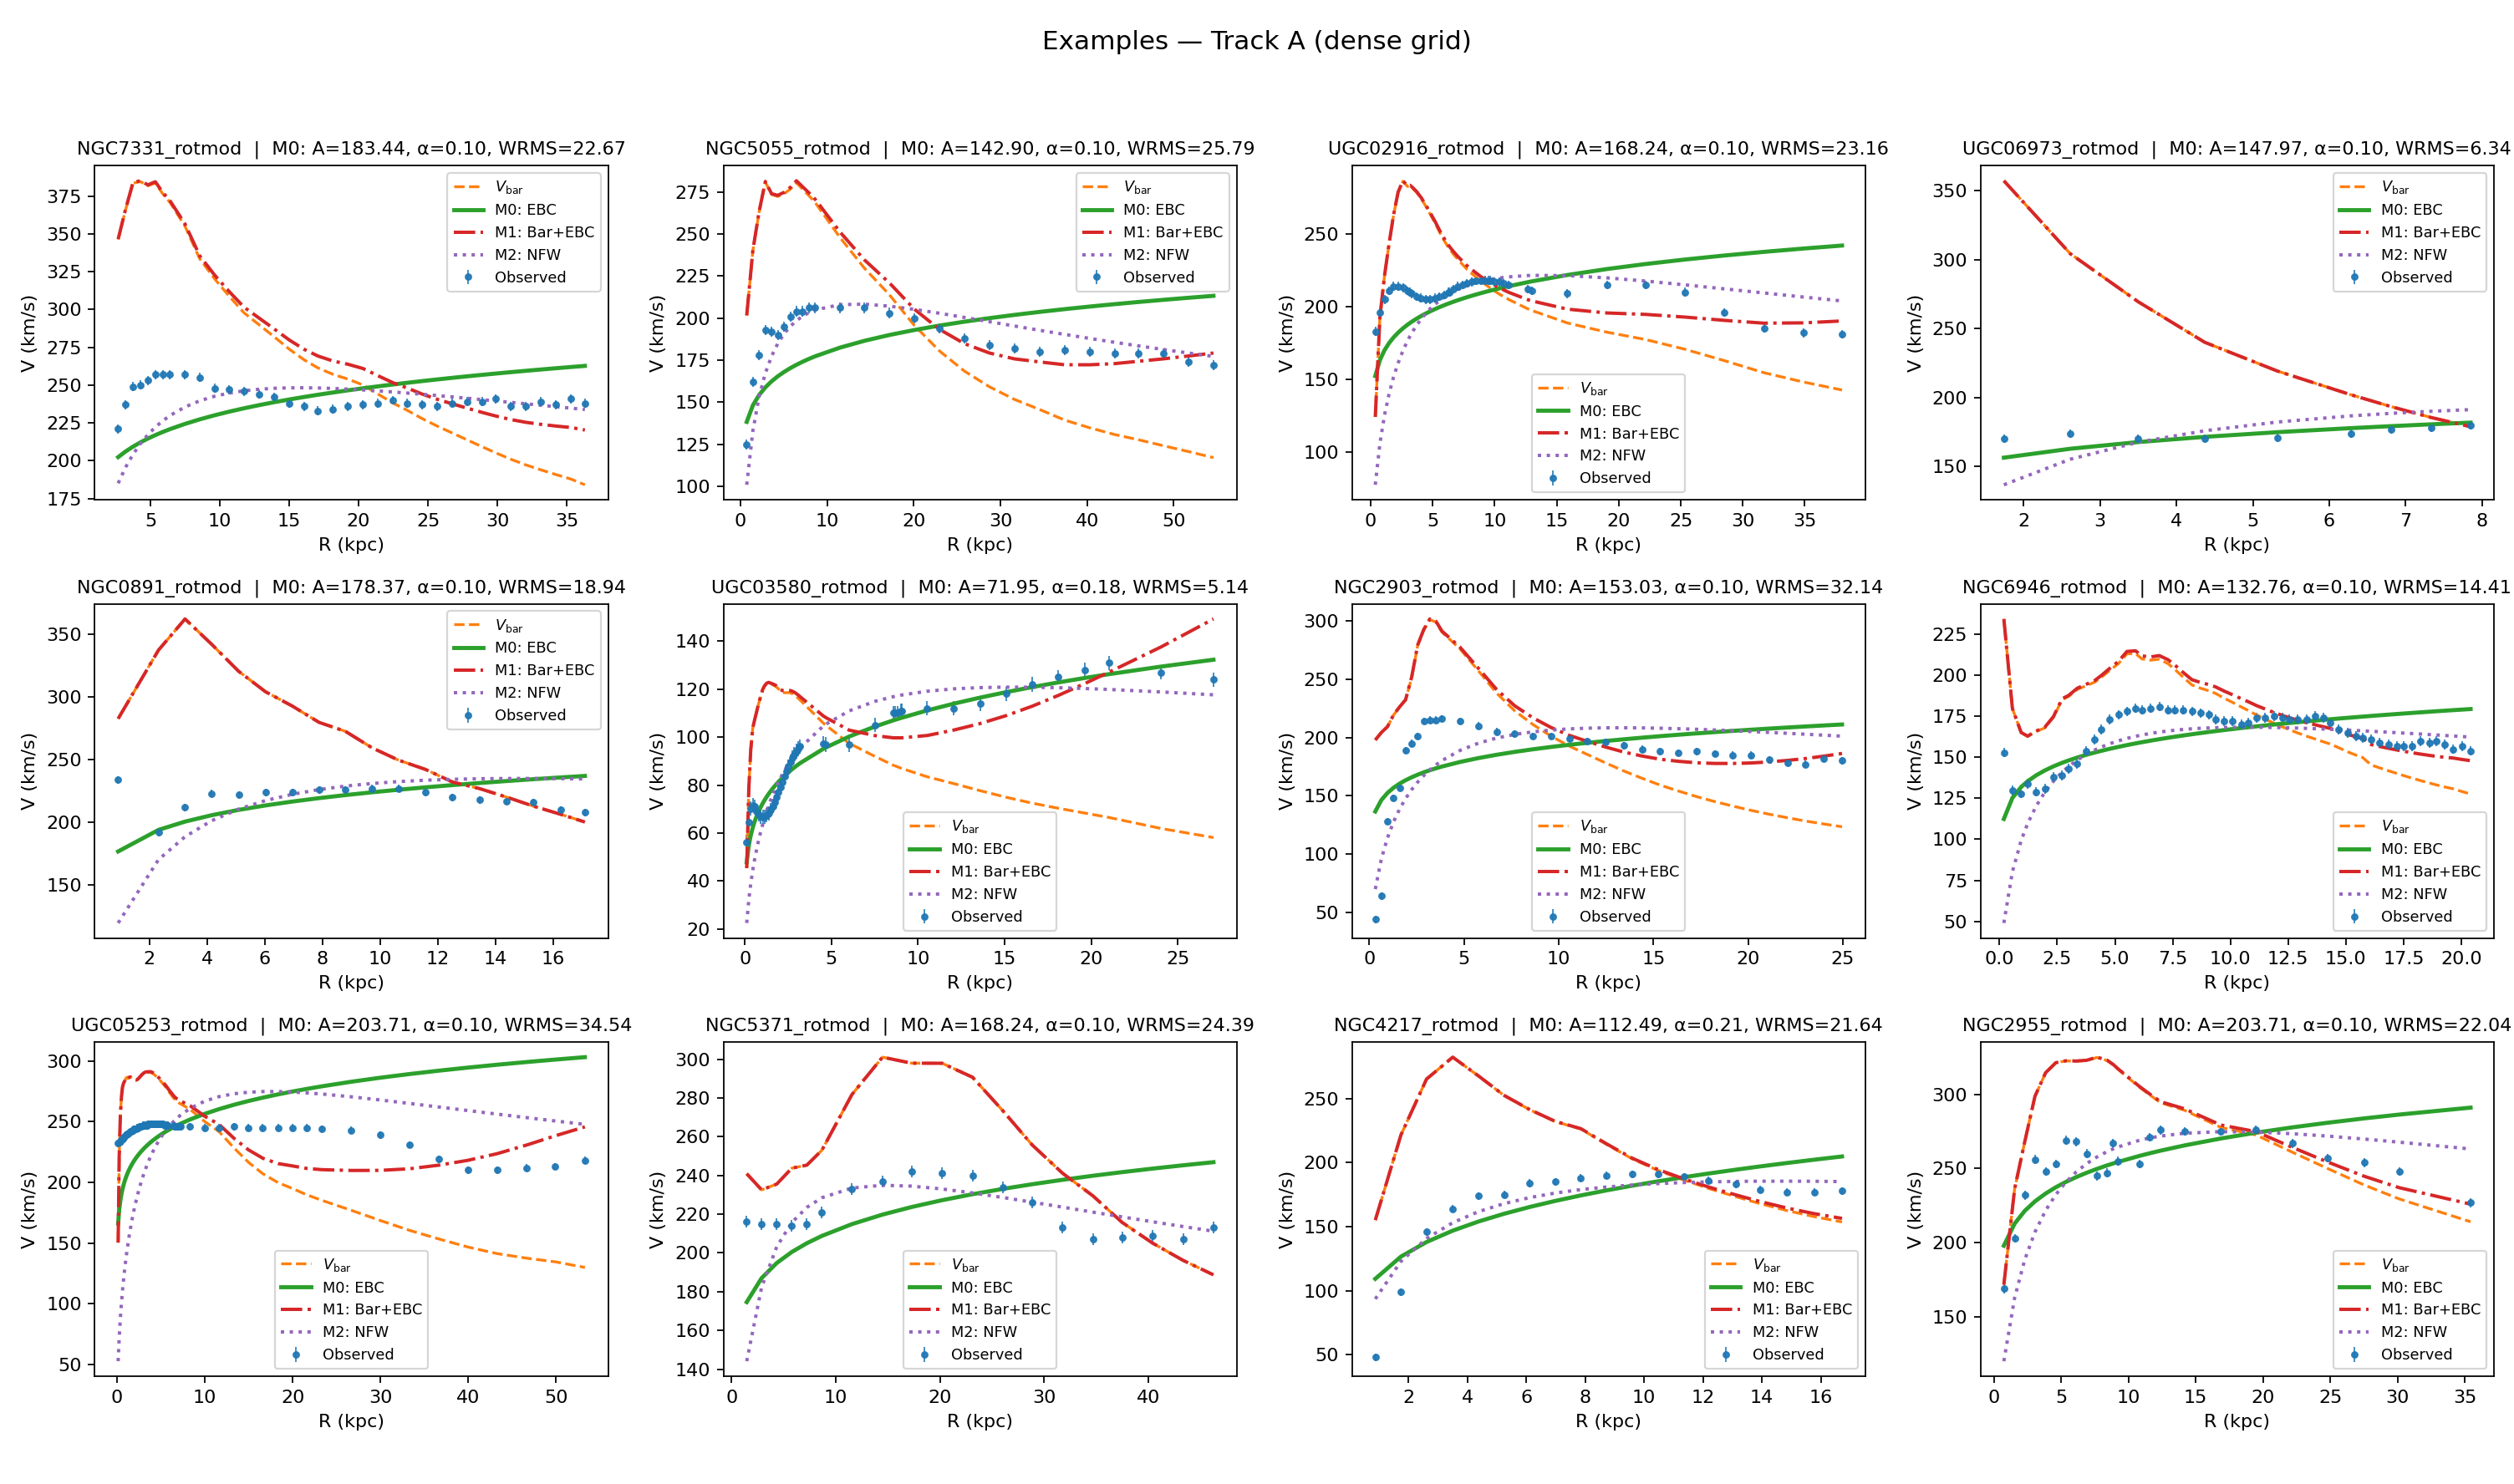
\includegraphics[width=\linewidth]{figs_m0_examples/trackA_dense_all/galaxy_parade_all.png}
  \caption{Twelve illustrative galaxies (Track A, dense grids). Orange dashed: $\Vbar$; green: M0 (EBC); red dash‑dot: M1 (Bar+EBC); purple dotted: M2 (Bar+NFW); points: observed.}
\end{figure}

\begin{figure}[H]
  \centering
  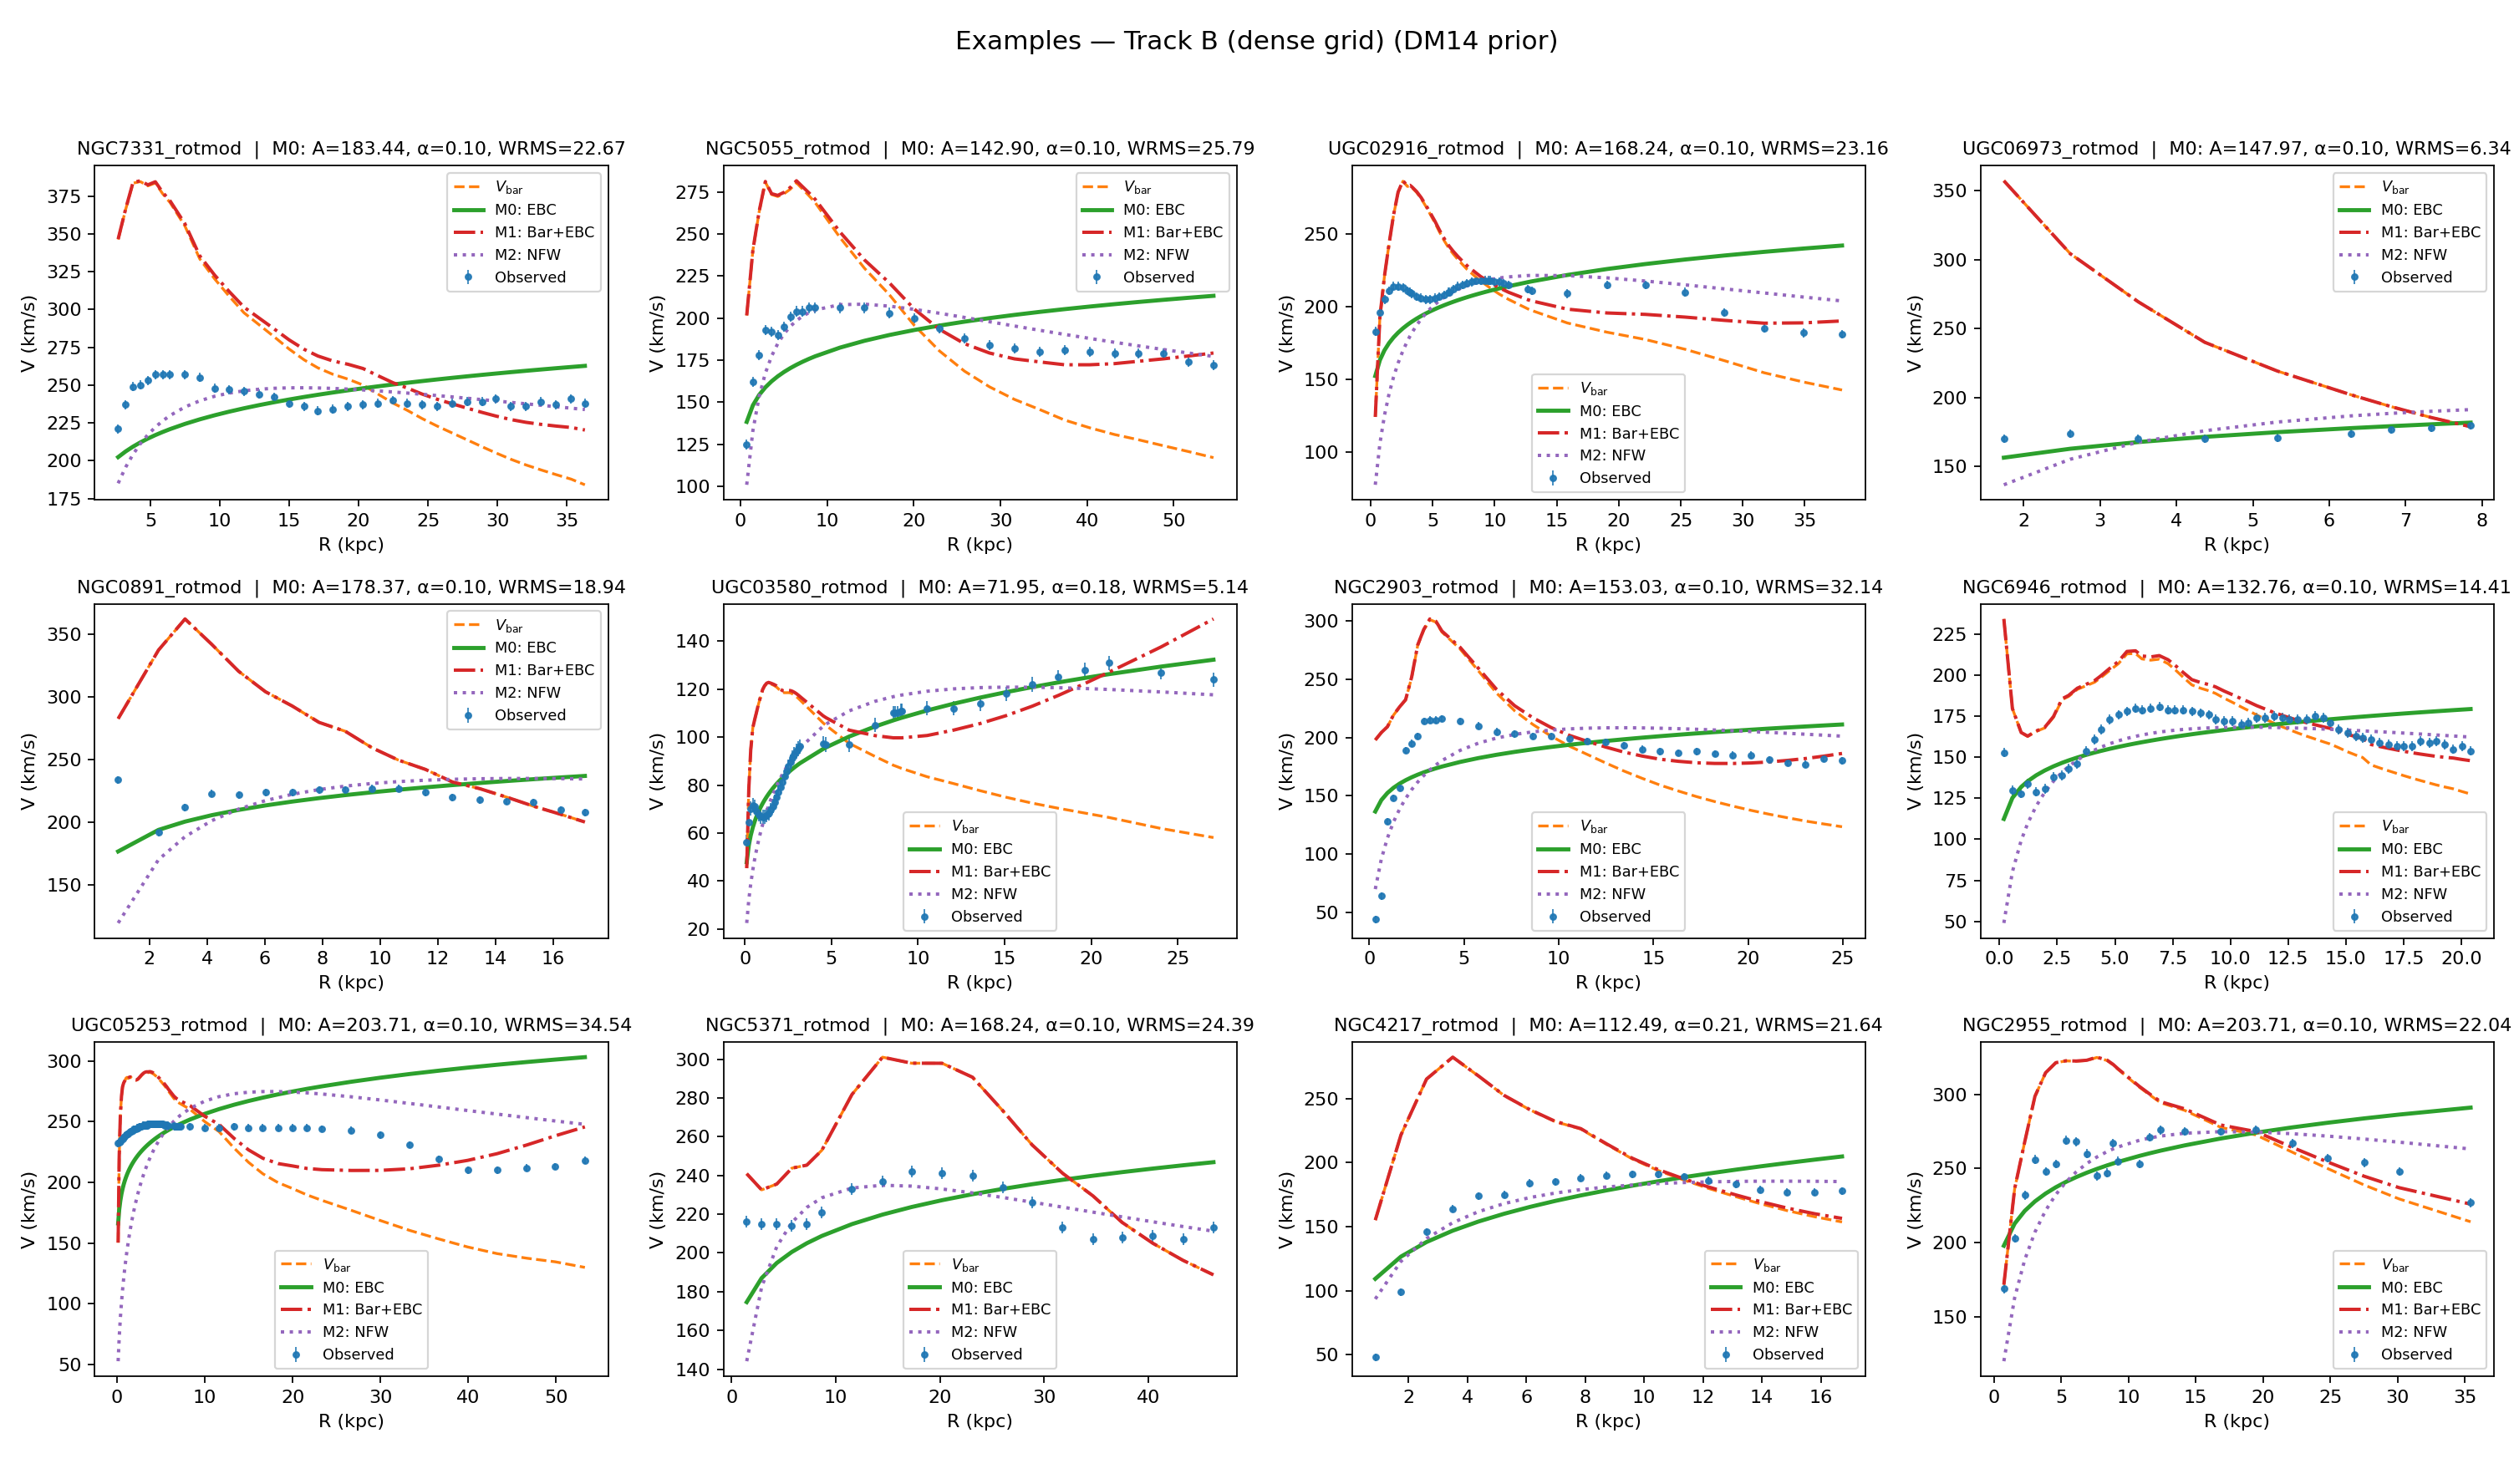
\includegraphics[width=\linewidth]{figs_m0_examples/trackB_dense_all/galaxy_parade_all.png}
  \caption{Twelve illustrative galaxies (Track B, dense grids with DM14 prior). Line styles as in Appendix Figure A1.}
\end{figure}

\section*{Appendix B: Reproducibility checklist (abbrev.)}
\begin{itemize}\itemsep0.2em
\item \textbf{Winner tables/$\Delta$BIC}: run \texttt{scripts/ebc\_ic\_referee.py} with Track A and Track B settings (dense symmetric grids, $\sigma$‑floor \SI{3}{\kms}, CV=5).
\item \textbf{CV boxplots}: \texttt{scripts/make\_cv\_boxplots.py} produces the PNG/SVG shown in Fig.~\ref{fig:cvbox}.
\item \textbf{Example overlays}: \texttt{scripts/plot\_examples\_overlay.py} with \texttt{--curves all} produces Appendix figures.
\item \textbf{QC‑failed (too few usable points, either track)}: D512‑2\_rotmod, F567‑2\_rotmod, F574‑2\_rotmod, NGC6789\_rotmod, UGC00634\_rotmod, UGC00891\_rotmod, UGC02023\_rotmod, UGC05999\_rotmod, UGC07232\_rotmod, UGC09992\_rotmod.
\end{itemize}

% =========================================================
\begin{thebibliography}{99}

% Core RC / paradigms
\bibitem{NFW1996} Navarro, J.~F., Frenk, C.~S., \& White, S.~D.~M. 1996, \emph{ApJ}, 462, 563.
\bibitem{NFW1997} Navarro, J.~F., Frenk, C.~S., \& White, S.~D.~M. 1997, \emph{ApJ}, 490, 493.
\bibitem{Planck2018} Planck Collaboration. 2018, \emph{A\&A}, 641, A6.
\bibitem{deBlok2001} de Blok, W.~J.~G., McGaugh, S.~S., \& Rubin, V.~C. 2001, \emph{AJ}, 122, 2396.
\bibitem{Gentile2004} Gentile, G., Salucci, P., Klein, U., \& Granato, G. 2004, \emph{MNRAS}, 351, 903.
\bibitem{Oman2015} Oman, K.~A., et al. 2015, \emph{MNRAS}, 452, 3650.
\bibitem{Milgrom1983} Milgrom, M. 1983, \emph{ApJ}, 270, 365.
\bibitem{McGaugh2020} McGaugh, S. 2020, \emph{Galaxies}, 8, 35.
\bibitem{McGaugh2016RAR} McGaugh, S., Lelli, F., \& Schombert, J. 2016, \emph{Phys. Rev. Lett.}, 117, 201101.
\bibitem{Lelli2016SPARC} Lelli, F., McGaugh, S., \& Schombert, J. 2016, \emph{AJ}, 152, 157.
\bibitem{DuttonMaccio2014} Dutton, A.~A., \& Macci\`o, A.~V. 2014, \emph{MNRAS}, 441, 3359.

% Halo profiles / priors / alternatives
\bibitem{Burkert1995} Burkert, A. 1995, \emph{ApJL}, 447, L25.
\bibitem{Navarro2004} Navarro, J.~F., et al. 2004, \emph{MNRAS}, 349, 1039.
\bibitem{Bullock2001} Bullock, J.~S., et al. 2001, \emph{MNRAS}, 321, 559}.
\bibitem{Maccio2008} Macci\`o, A.~V., et al. 2008, \emph{MNRAS}, 391, 1940.
\bibitem{deBlok2010} de Blok, W.~J.~G. 2010, \emph{Advances in Astronomy}, 2010, 789293.

% Information criteria / CV / Jeffreys
\bibitem{Akaike1974} Akaike, H. 1974, \emph{IEEE Trans. Autom. Control}, 19, 716.
\bibitem{Sugiura1978} Sugiura, N. 1978, \emph{Commun. Stat. A}, 7, 13.
\bibitem{Schwarz1978} Schwarz, G. 1978, \emph{Ann. Stat.}, 6, 461.
\bibitem{KassRaftery1995} Kass, R.~E., \& Raftery, A.~E. 1995, \emph{JASA}, 90, 773.
\bibitem{Jeffreys1961} Jeffreys, H. 1961, \emph{Theory of Probability}, 3rd ed., Oxford Univ. Press.
\bibitem{Stone1974} Stone, M. 1974, \emph{J. Roy. Stat. Soc. B}, 36, 111.
\bibitem{ArlotCelisse2010} Arlot, S., \& Celisse, A. 2010, \emph{Statistics Surveys}, 4, 40.

% Classic rotation-curve / mass modeling
\bibitem{Begeman1991} Begeman, K.~G., Broeils, A.~H., \& Sanders, R.~H. 1991, \emph{MNRAS}, 249, 523.
\bibitem{deBlokBosma2002} de Blok, W.~J.~G., \& Bosma, A. 2002, \emph{A\&A}, 385, 816.

% Software stack
\bibitem{NumPy} Harris, C.~R., et al. 2020, \emph{Nature}, 585, 357.
\bibitem{SciPy} Virtanen, P., et al. 2020, \emph{Nat. Methods}, 17, 261.
\bibitem{Matplotlib} Hunter, J.~D. 2007, \emph{Computing in Science \& Engineering}, 9, 90.

% Companion theory (optional, clearly labeled)
\bibitem{Tupay2025b} Tupay, J.~A.~M. 2025, \emph{A Complete Theoretical Framework for Power-Law Galactic Rotation Curves: From Tsallis Non-Extensive Statistics to Observable Predictions}, submitted.
\end{thebibliography}

\end{document}